%% The '3p' and 'times' class options of elsarticle are used for Elsevier CRC
\documentclass[3p,times]{elsarticle}

%% set the volume if you know. Otherwise `00'
%\volume{00}

%% set the starting page if not 1
%\firstpage{1}

%% Give the name of the journal
%\journalname{Journal of Systems and Software}

%% Give the author list to appear in the running head
%% Example \runauth{C.V. Radhakrishnan et al.}
%\runauth{S. Venkatanarayan et al.}

%% The choice of journal logo is determined by the \jid and \jnltitlelogo commands.
%% A user-supplied logo with the name <\jid>logo.pdf will be inserted if present.
%% e.g. if \jid{yspmi} the system will look for a file yspmilogo.pdf
%% Otherwise the content of \jnltitlelogo will be set between horizontal lines as a default logo

%% Give the abbreviation of the Journal.
%\jid{JSS}

%% Give a short journal name for the dummy logo (if needed)
%\jnltitlelogo{Journal of Systems and Software}

%% Hereafter the template follows `elsarticle'.
%% For more details see the existing template files elsarticle-template-harv.tex and elsarticle-template-num.tex.

%% Elsevier CRC generally uses a numbered reference style
%% For this, the conventions of elsarticle-template-num.tex should be followed (included below)
%% If using BibTeX, use the style file elsarticle-num.bst

%% End of ecrc-specific commands
%%%%%%%%%%%%%%%%%%%%%%%%%%%%%%%%%%%%%%%%%%%%%%%%%%%%%%%%%%%%%%%%%%%%%%%%%%

\usepackage{url}
\usepackage{listings}
\usepackage{subfig}
\usepackage{todo}
\usepackage{mdframed}
\usepackage{xcolor}
\usepackage{colortbl}
\definecolor{verylightgray}{gray}{0.7}
\usepackage{url}
\usepackage{tikz}
\tikzstyle{block} = [rectangle, draw, 
    text width=5em, text centered, rounded corners, minimum height=2em]
\tikzstyle{oval} = [ellipse, draw, 
    text width=5em, text centered, rounded corners, minimum height=2em]
\tikzstyle{bt} = [rectangle, draw, 
    text width=1em, text centered, rounded corners, minimum height=2em]
\usetikzlibrary{calc}
\usetikzlibrary{arrows.meta}
\usetikzlibrary{positioning}
\usetikzlibrary{fit}
\usetikzlibrary{shapes.geometric}

\usepackage{inconsolata}
\lstset{basicstyle=\ttfamily}


%% The amssymb package provides various useful mathematical symbols
\usepackage{amssymb}
%% The amsthm package provides extended theorem environments
%% \usepackage{amsthm}

%% The lineno packages adds line numbers. Start line numbering with
%% \begin{linenumbers}, end it with \end{linenumbers}. Or switch it on
%% for the whole article with \linenumbers after \end{frontmatter}.
%% \usepackage{lineno}

%% natbib.sty is loaded by default. However, natbib options can be
%% provided with \biboptions{...} command. Following options are
%% valid:

%%   round  -  round parentheses are used (default)
%%   square -  square brackets are used   [option]
%%   curly  -  curly braces are used      {option}
%%   angle  -  angle brackets are used    <option>
%%   semicolon  -  multiple citations separated by semi-colon
%%   colon  - same as semicolon, an earlier confusion
%%   comma  -  separated by comma
%%   numbers-  selects numerical citations
%%   super  -  numerical citations as superscripts
%%   sort   -  sorts multiple citations according to order in ref. list
%%   sort&compress   -  like sort, but also compresses numerical citations
%%   compress - compresses without sorting
%%
%% \biboptions{comma,round}

% \biboptions{}

% if you have landscape tables
\usepackage[figuresright]{rotating}

% put your own definitions here:
%   \newcommand{\cZ}{\cal{Z}}
%   \newtheorem{def}{Definition}[section]
%   ...

% add words to TeX's hyphenation exception list
%\hyphenation{author another created financial paper re-commend-ed Post-Script}

% declarations for front matter

\begin{document}

\begin{frontmatter}

%% Title, authors and addresses

%% use the tnoteref command within \title for footnotes;
%% use the tnotetext command for the associated footnote;
%% use the fnref command within \author or \address for footnotes;
%% use the fntext command for the associated footnote;
%% use the corref command within \author for corresponding author footnotes;
%% use the cortext command for the associated footnote;
%% use the ead command for the email address,
%% and the form \ead[url] for the home page:
%%
%% \title{Title\tnoteref{label1}}
%% \tnotetext[label1]{}
%% \author{Name\corref{cor1}\fnref{label2}}
%% \ead{email address}
%% \ead[url]{home page}
%% \fntext[label2]{}
%% \cortext[cor1]{}
%% \address{Address\fnref{label3}}
%% \fntext[label3]{}

%\dochead{}
%% Use \dochead if there is an article header, e.g. \dochead{Short communication}

  \title{Design and implementation of the VizAPI tool: a case study for static and dynamic analysis of Java plus visualization}

%  Design and implementation of the VizAPI tool: s
  
%% use optional labels to link authors explicitly to addresses:
%% \author[label1,label2]{<author name>}
%% \address[label1]{<address>}
%% \address[label2]{<address>}

\author{Sruthi Venkatanarayanan}
\author{Craig Anslow}
\author{Patrick Lam}

\address{}

\begin{abstract}
  The VizAPI tool shows visualizations that include both static and dynamic interactions between clients, the libraries they use, and those libraries’ transitive dependencies (as long as the components are in Java). Client developers can use VizAPI to answer a query about upstream code: will their code be affected by breaking changes in library APIs? Or, library developers can use VizAPI to find out about downstream code: which APIs in their source code are commonly used by clients?

In this paper, we describe the design and implementation of VizAPI, including our approach to static and dynamic analysis using the Javassist library. We focus on artifact-level issues: to help future program analysis tool developers, we discuss viable alternative libraries that we could have used to implement this tool. We then explain how we collected a dataset for VizAPI consisting of 11 libraries and 90 clients, transitively including 4297 components in all. Finally, we discuss potential future uses of VizAPI.
\end{abstract}

\begin{keyword}
static program analysis \sep
dynamic program analysis \sep
API usage \sep
software evolution \sep
software maintenance
%% keywords here, in the form: keyword \sep keyword

%% MSC codes here, in the form: \MSC code \sep code
%% or \MSC[2008] code \sep code (2000 is the default)

\end{keyword}

\end{frontmatter}

%%
%% Start line numbering here if you want
%%
% \linenumbers

%% main text
\section{Introduction}
\label{sec:introduction}



The submitted papers should describe the artefact and its potential uses for other researchers.


Goal (why did we produce this data?):
investigate API usage patterns, both conceptually and in practice

Dimensions of data: what, how, which way, why not (section 2.1 in thesis)



\section{VizAPI Implementation}
\label{sec:implementation}
We now describe VizAPI which includes two phases: (1) data extraction and (2) visualizations. 

The data extraction phase uses static and dynamic
analysis to collect data about client usages of libraries. We generate both static and
dynamic call graphs, and we also capture other client-library interactions. The static analysis captures the
following interactions: vanilla invocations, field accesses, class usages,
setAccessible(), annotations and inheritance information. The dynamic
analysis captures all dynamic uses of those patterns and additionally
reflection, dynamic proxies and service loader bypasses.

The visualization phase transforms the data extracted in the first phase into d3 format by first converting the data into a graph and then using our customized version
of the d3graph\footnote{\url{https://pypi.org/project/d3graph/}} library in Python to generate d3js\footnote{\url{https://d3js.org/}} visualizations. 

In this section, we start by describing VizAPI. Next, we discuss its implementation. Then, in Section~\ref{sec:design-decisions}, we explore
alternatives that we could have chosen, including their advantages and
drawbacks.  The goal of this paper is to produce an explanation of our
artifact that will be helpful to other researchers, including in
particular an exploration of the design space for program analysis and visualization tools like ours.

\subsection{Overview}
We briefly give an overview of VizAPI to enable discussions of its design and implementation.
The VISSOFT paper~\cite{venkatanarayanan22:_vizap}
and the first author's MMath thesis~\cite{venkatanarayanan22:_study_lever_api_usage_patter} explains VizAPI in more detail.

We first define the terms ``client'', ``library'', ``dependency'' and ``interaction", which we use throughout this paper. A ``client'' is a software component which directly uses some functionality of an external component, which is the ``library''. Any external component that the ``library'' directly uses is a ``dependency'' of that library; components may also have ``transitive dependencies''. The pattern observed when a client/library boundary is crossed is an ``interaction". Examples of interactions include vanilla invocations, field accesses and annotation usage.

VizAPI creates graphs where the nodes are packages that belong to components (clients, libraries and dependencies) and the edges represent the types of interactions between the packages. We create these graphs with the goal of being useful to developers who are thinking about API design questions for their clients and libraries.

\begin{figure}[h]
\begin{center}
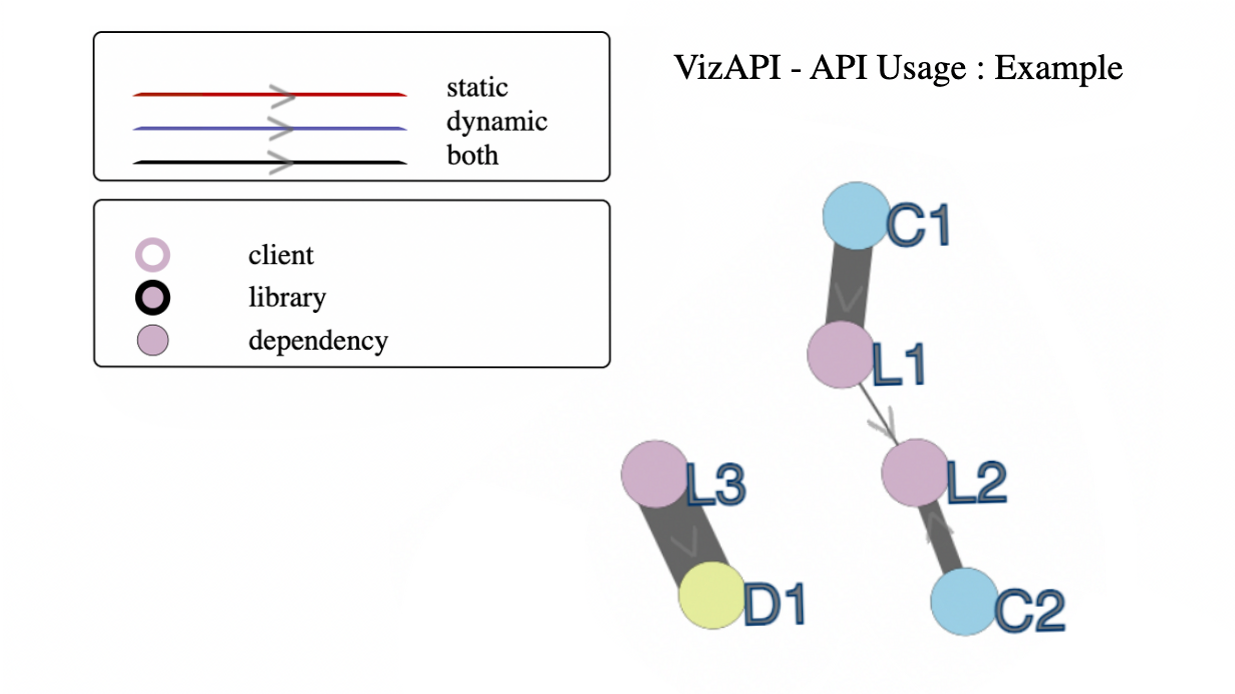
\includegraphics[height=4cm,width=7cm]{images/intro-example.png}
\caption{VizAPI visualization of client C which calls library L, itself dependent on dependency D.}
\label{fig:example}
\end{center}
\end{figure}

Figure~\ref{fig:example} illustrates a VizAPI usage scenario, from the perspective of a client developer worried about breaking changes from a new version of a library. It shows Java client $C$ (blue nodes) and library $L$ (purple nodes). Library $L$ has packages $L_1$, $L_2$, and $L_3$. $C$ calls into $L_1$ and $L_2$. Internally, within $L$, $L_1$ and $L_2$ call into each other, but not into $L_3$. The VizAPI result, with no edges from $C$ directly to $L_3$, allows a developer to conclude that breaking changes in $L_3$ will not affect $C$. Also, if only $L_3$ uses an external dependency $D$ (yellow node), then $C$ will not need $D$ to be on its classpath.

To produce its graphs, VizAPI needs to collect information about interactions between clients, libraries, and dependencies. We provide a few examples of interactions---enough to give the idea of what VizAPI is looking for, but not an exhaustive list.

\paragraph{Vanilla invocations} The goal here is to capture information about method calls between components. This information can be approximated statically using Class Hierarchy Analysis, as we describe below. Furthermore, it can also be captured precisely at runtime, at least for the invocations that happens on a particular set of executions.

\paragraph{Dynamic proxies and reflective calls} We use a dynamic approach for recording calls made using Java dynamic proxies and Java reflection to avoid needing to make hopelessly conservative approximations. The soundiness manifesto~\cite{livshits15:_in_defen_sound} points out that many papers in the literature claim soundness and are, in fact, sound for most language features, but exclude highly dynamic features like reflection. VizAPI uses dynamic information and instrumentation to capture certain patterns of reflection and dynamic proxies.

\paragraph{Service Loaders} This Java API allows Java programs to dynamically load additional code, typically plugins. The plugins would declare a published interface, which we can record statically. VizAPI captures uses of the published interface as well as dynamic calls that exceed the public interface.


\subsection{Overall Design of VizAPI}
We now explain the design of our VizAPI tool, which integrates data from both static and dynamic analysis.
We use Javassist~\cite{chiba00:_load_struc_reflec_java} for our static analysis, which we discuss in Section~\ref{subsec:static}. We also use Javassist to instrument the code so that we can
collect dynamic analysis data; we discuss that part in
Section~\ref{subsec:dynamic}.

Our static and dynamic analysis tool takes in a set of clients and libraries as input.
We programatically obtain a list of dependencies for each client and library by invoking Maven, and locate the JARs that Maven downloads in its build output.
We first record the extents of components (clients, libraries, and dependencies) by inspecting JAR
files of each software component to obtain a
list of classes for that component. We associate classes and their
members to components based on these lists.  This allows us to
identify interactions across the client/library boundaries (i.e. between classes that appear on different lists).
Using Maven, we build JAR
files that contain source code only. This ensures that we do not
capture library uses meant solely for unit testing. 

Figure~\ref{fig:workflow} summarizes our
(static) data capture and (dynamic) instrumentation workflow.  \\

\begin{figure*}[h]
 \begin{center}
\resizebox{0.9\textwidth}{!}{
  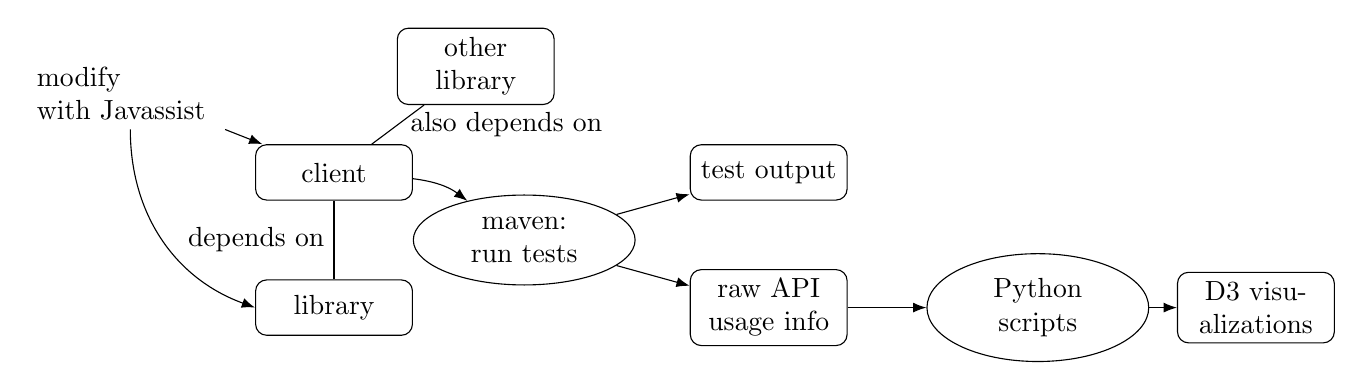
\begin{tikzpicture}
    \node[block] (client) {client};
    \node[block,below=1cm of client] (library) {library};

    \draw (library) -- node[left] (depends) {depends on} (client);

    \node[above left=.75em of client] (ja) {\begin{minipage}{7em} modify \\with Javassist \end{minipage}};
    \draw[-Latex] (ja) -> (client);
    \draw[-Latex] (ja) to [->,bend right=35] (library.west);

    \node[block, above right=2em of client,xshift=-2em] (olib) {other library};
    \draw (client) -- node[right,xshift=.1em] (also) {also depends on} (olib);

    \node[oval,right=of depends] (test) {maven: run tests};

    \draw[-Latex] (client) to [->,bend left=15] (test);

    \node[block, right=10em of client] (output) {test output};
    \node[block, right=10em of library] (raw) {raw API usage info};

    \draw[-Latex] (test) to (output);
    \draw[-Latex] (test) to (raw);

    \node[oval, right=of raw] (Py) {Python scripts};
    \draw[-Latex] (raw) to (Py);

    \node[block, right=1em of Py] (viz) {D3 visualizations};
    \draw[-Latex] (Py) to (viz);
  \end{tikzpicture}
}
  \caption{Our instrumentation workflow. Using Javassist, we analyze and instrument clients and run their test suites. (We process the generated data with Python scripts to create D3 visualizations for VizAPI.)}
  \label{fig:workflow}
 \end{center}
\end{figure*}



\subsection{Static Analysis}
\label{subsec:static}
It turns out that a simple (rather straightforward) static analysis suffices
for our purposes, and we describe parts of it in this section. Section~\ref{sec:design-decisions}
discusses when the use of more sophisticated analyses is appropriate, and
how to incorporate such analyses in an analysis pipeline.

For VizAPI, using Javassist, we 
perform class hierarchy analysis on components and create a static call
graph. 

We implement class hierarchy analysis ourselves. We first read the class files from JARs of clients, libraries, and dependencies (provided by Maven) and we record
inheritance relationships between classes. Then, when we walk through the different kinds of interactions,
 we add an edge between the caller and its potential callees---because we use Class Hierarchy Analysis, the set of potential callees follows from the recorded inheritance relationships.
Some of the interactions we record include vanilla invocations, subtyping and annotations.

\paragraph{Vanilla invocations}
The standard case is simple. At every invoke instruction in every
loaded method which transfers control between a client and a
library, we record a static dependency using the class hierarchy
analysis call graph that we compute.

\paragraph{Subtyping}
We record information about all superclasses and implemented interfaces that cross the library/client barrier. 

\paragraph{Annotations}
We have a quasi-static approach for finding class, field and method annotations:
we observe all annotations for a class or class member when it is loaded, and
record cases where a class or member declares an annotation from the library of interest.

\subsection{Dynamic Analysis}
\label{subsec:dynamic}
We collect dynamic data about client usages of libraries by running client
test suites under instrumentation. The instrumentation records API
uses which cross client/library boundaries, closely mirroring the API
usage patterns
in~\cite{venkatanarayanan22:_study_lever_api_usage_patter}. We first
describe how we capture specific dynamic interactions between components, and
then discuss our instrumentation implementation.

\paragraph{Vanilla invocations} 
At every invoke instruction in every
loaded method which transfers control between a client and a
library, we add code to dynamically record
the invoke by incrementing a counter just before the invoke
executes. Note that we handle all Java invocation types, including
virtual and even dynamic invokes. Crossing the client/library boundary
includes conventional calls from the client to the library as well as
callbacks from the library to the client.  Because we instrument
libraries, we can record both invocation directions.

\paragraph{Dynamic proxies and reflective calls}
Our instrumentation intercepts calls to
\texttt{java.lang.reflect.Method.invoke()}, a distinguished method
used to invoke dynamic proxies and reflective calls, 
recording details of the calls that we intercept at runtime. It is possible for
static analyses to resolve a subset of such calls using advanced
techniques~\cite{christensen03:_precis_analy_strin_expres}. Our static analysis machinery does not provide enough information to
statically resolve this dependency, but we have full visibility on
calls that actually happen dynamically.

\paragraph{Service Loaders} Before the instrumentation, we record a list 
of services and their implementations by statically inspecting files in \texttt{src/main/resources/META-INF/services}. 
This gives a static list of dependencies; anything beyond this list that we observe dynamically would be a service bypass. 
In the dynamic phase, we use the statically recorded information to dynamically detect service bypasses which are direct uses of service implementation 
classes in clients, either through instantiations, casts or reflection. To do so, we intercept calls 
to method \texttt{load()} in classes with name \texttt{Service*Loader} and record any calls to methods beyond 
the published interface that we have recorded statically.

%\paragraph{How we implemented instrumentation}
\paragraph{Instrumentation}
In the dynamic analysis phase, we modify the build system of each
client (we chose clients that all use Maven) to run its provided unit tests on instrumented code.
Asking the modified build system to run the client's tests gives us dynamic call graphs as a side-effect output.

Specifically, using the Java instrumentation APIs and getting them to call Javassist APIs that modify bytecode,
we instrument classes and their members to increment counters for every interaction source
with a destination lying outside the JAR that it belongs to.
Our system creates code to carry out instrumentation and places it into a Java agent JAR.
The agent is then passed as an argument to Maven when running client unit tests, which attaches it to the JVM.
Once classes are loaded, the agent modifies the bytecode and it is then executed.
The code that we insert during the instrumentation phase keeps track of interactions and counters,
and writes them out upon program termination. \\


While our current benchmark set consists of 101 projects, it is possible to run both our static and dynamic analysis tool and the VizAPI visualization tool on new libraries and clients. However, when a library developer wishes to use VizAPI, they are required to provide a specific set of clients that they wish to observe as input to the tools. Developers can use libraries.io to find popular clients of libraries---it provides a dependency tree based on projects' packaging information.


\subsection{Visualizations}
\label{subsec:vis-system}

\begin{figure*}[h]
\begin{center}

\subfloat[Usage Scenario 1: Library \textit{jsoup} (pink with dark borders), called by two clients, \textit{ez-vcard} (hollow with purple border) and \textit{JsoupXpath} (hollow with pink border). Exploration shows that internal jsoup packages aren't called directly by clients.
\label{fig:usagescenario1}]
{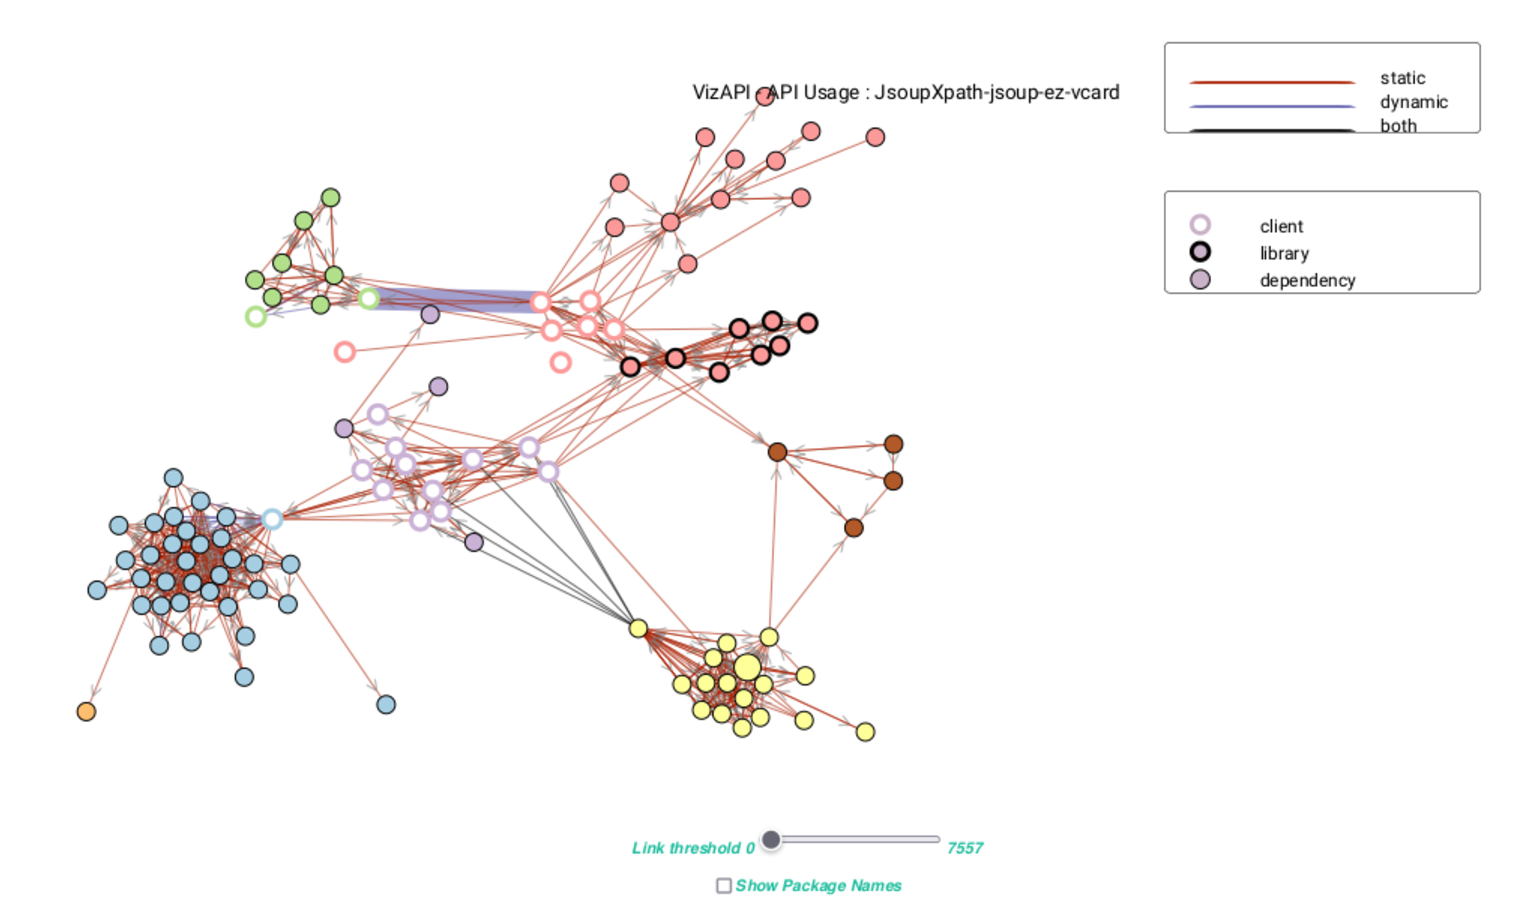
\includegraphics[width=16cm]{images/usage-scenario1.pdf}}
\hspace{7mm}

\subfloat[Usage Scenario 2: Client \textit{dataprocessor} (hollow, orange border) calls only one package in library \textit{fastjson} (green fill).
\label{fig:usagescenario2}]
{
\makebox[16cm]{
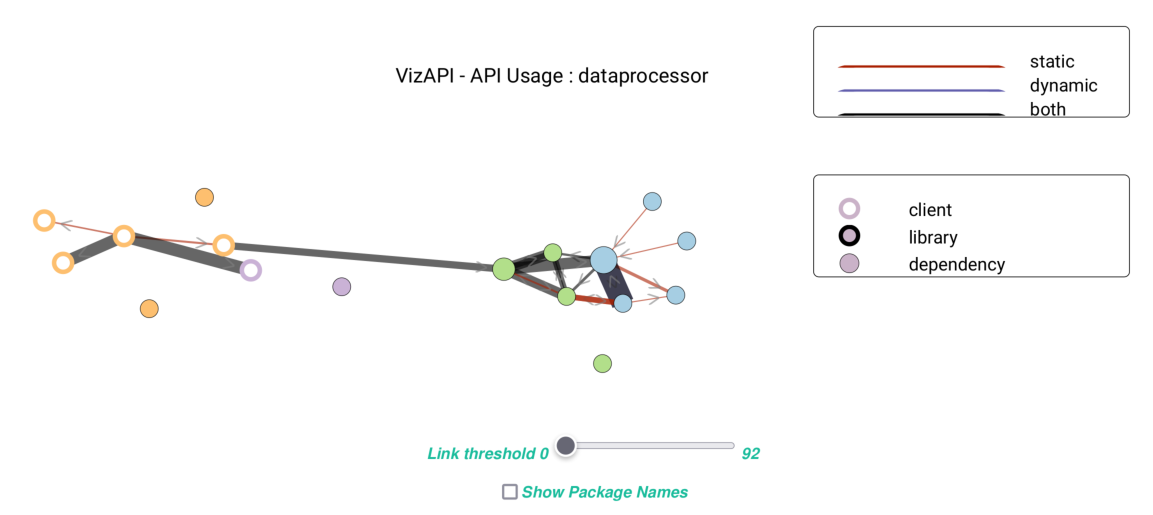
\includegraphics[width=11cm]{images/usage-scenario2.pdf}
}
}
\caption{\label{fig:usagescenarios} VizAPI Usage Scenarios.}

\end{center}
\end{figure*}


Once we have generated static and dynamic analysis data using our tool, we use a modified version
of the d3graph\footnote{\url{https://pypi.org/project/d3graph/}} library in Python to generate a d3js\footnote{\url{https://d3js.org/}}
visualization. The modifications that we made to the d3graph  library in Python include styling changes (for example, changing node styles based on whether it is a client, library or dependency),
legends, and a toggle to show all package names. 
The graphs in Figures~\ref{fig:example}, \ref{fig:usagescenario1}, and \ref{fig:usagescenario2} are examples of graphs produced by VizAPI.

VizAPI graphs are force-directed graphs based on the frequency of
interactions between different software components. 
Here, frequency of interactions indicates the sum of number of times different kinds of interactions occur.
Each node is a
set of one or more packages that belong to the same JAR.  There are
three categories of nodes: clients are represented by nodes with white
interiors; libraries by nodes with filled interiors and black borders;
and dependencies (called by libraries but not clients) by nodes with
filled interiors and normal borders.  We coalesce nodes if they
originate from the same JAR and have the same incoming and
outgoing edges.

Each edge is directed
from the source package(s) to the target package(s) and represents an interaction 
(e.g. invocations, fields, annotations, subtyping) between packages. 
The thickness of each edge reflects the frequency of interactions between the source and the target.
Double-clicking on a node emphasizes its direct interactions with other packages while fading out the rest of the graph.
To search for a package, the user can click on ``show package
names'' and use the browser’s find functionality. 
The ``Link threshold'' slider allows the user to form new clusters based on frequencies of interactions.


We run a Python implementation of the Louvain clustering algorithm~\cite{blondel2008fast}, and make the clusters 
visible by colouring nodes based on cluster.
Nodes of the same cluster may come from the same or different JARs.
Hovering on a node shows the list of packages and 
the JAR that they belong to, 
formatted as ``jar : $\langle$space separated list of packages$\rangle$''. 
Hovering on an edge shows the type of interaction (invocations, fields, annotations, subtyping or a combination of these) between nodes.

\section{Design Decisions}
\label{sec:design-decisions}

Soundiness and the combined static/dynamic approach

\subsection{Static analysis}
In terms of static analysis, we describe potential approaches going
from low-level bytecode manipulation through to declaratively declaring
desired analysis facts.

At the intraprocedural level, most tools provide access to bytecode
manipulation. Some tools allow users to supply Java code which is
then compiled into bytecode. Soot has an intermediate three-address code.

Working at the bytecode level imposes unnecessary complexity on
static analyses. See early Soot papers for details.

Javassist, BCEL, ASM

cglib

ByteBuddy


DiSL https://link.springer.com/chapter/10.1007/978-3-642-35182-2_18

https://stackoverflow.com/questions/9167436/dynamic-java-bytecode-manipulation-framework-comparison



SCAM21 submission on mocks


Drivers

\paragraph{Pointer analysis and callgraphs.}

Pointer analysis: haven't we solved this problem already? (Hind, 20 years ago).

CHA: simplest possible option

RTA

Demand-driven approaches

Object-sensitive

Soundiness

\paragraph{Going interprocedural}
Assuming that we have a call graph available, the next challenge in
designing a tool is to correctly propagate data interprocedurally.
Even with Soot's call graph informatoin, it is still not that easy to
do whole-program analyses: it is up to the user to manually propagate
information at method invocation sites.

Heros implements IFDS/IDE for interprocedural analysis.
It's more complicated to use than intraprocedural analysis.

As an alternative to Heros, Doop enables its users to state
declarative facts. It then uses solvers to compute the solution over the
entire program. The pointer analysis to be used is a parameter.

Runtime of Soot versus Doop and Heros.


\subsection{Dynamic analysis}

java agent versus JVMTI

Code rewriting


\section{Dataset}
\label{sec:benchmark}
We believe that information about our dataset collection process and the dataset itself will be useful to other researchers, and thus describe it in this section. Our benchmark set consists of 11 libraries and 90 clients. For libraries, we pick the most popular Maven 
repositories in different categories such as logging, JSON parsing and databases. While this is still a convenience sample, we aimed for some representativeness in categories and also some overlap (i.e. more than one entry per category).

Table~\ref{tab:libs} presents our set of libraries. We measured lines of code (kLOC) using SLOCcount\footnote{\url{https://dwheeler.com/sloccount/}} and number of classes by building libraries and counting resulting \texttt{.class}es. Since VizAPI aims to understand relationships between components, we classified component types as follows. A project uses ServiceLoaders if it has a \texttt{META-INF/services} directory and Java 9 modules if it has a \texttt{module-info.java} file. A library is an OSGi component if it contains a \texttt{MANIFEST.MF} file in its build output\footnote{Some libraries (for example, \emph{connector-j}) create OSGi metadata during the build, so we look for the metadata in the build output, not in the source.}, and this manifest contains \texttt{Export-Package} declarations. 

\begin{table}[h]
\begin{center}
\caption{\label{tab:libs}Libraries that we investigated for API usage and mis-usage patterns}
\begingroup\scriptsize	
\hspace*{-0.6cm}
\begin{tabular}{l!{\color{verylightgray}\vrule}cl!{\color{verylightgray}\vrule}rr!{\color{verylightgray}\vrule}ccc}
& & & non-test &  & Service & Java 9 &  \\
Library & version & description   & kLOC     & \# classes  &  Loader  & modules & OSGi \\ \arrayrulecolor{verylightgray}\hline
commons-collections4 & 4.4 & data structure implementations & 28.9 & 524 &&&\checkmark\\
commons-io & 2.8.0 & IO functionality library & 12.6 & 182& & &\checkmark\\
joda-time & 2.10.10 & date and time handling library & 28.9 & 247&&& \checkmark \\
slf4j-api & 1.7.9 & logging library & 1.5 & 28 & & & \checkmark\\
jsoup & 1.13.1 & HTML parser & 12.5 & 249&&&\checkmark\\
fastjson & 1.2.76 & JSON parser/generator & 43.6 & 260 &\checkmark&\\ 
gson & 2.8.8 & JSON parser/generator & 14.4&  182 && \checkmark&\checkmark\\
json & 20210307 & JSON parser/generator & 11.8 & 27& & \\
jackson-core & 2.12.3 & JSON parser/generator & 27.1 & 124 & \checkmark&  \checkmark&\\
jackson-databind & 2.12.3 & bindings for JSON parser/generator & 68.2 & 700 & \checkmark & \checkmark&\\ 
h2 & 1.4.200 & database & 147.2 & 1010 & \checkmark & & \checkmark \\
\end{tabular}
\endgroup
\end{center}
\end{table}

We use the libraries.io dataset\footnote{\url{https://libraries.io/}} to construct a dependency graph and look for the most used upstream components (highest number of other components depends on [any version of] those), 
and the top downstream components (clients). We exclude any clients that have fewer than 10 stars or fewer than 10 forks on Github.  Apart from this, we also pick a subset of projects from the
Duets benchmarks~\cite{durieux21}. We exclude components that do not contain unit tests, components that use our chosen library only for testing,
and components that declare the library as a dependency in their POM file, but do not actually use it. Our benchmark set contains both Maven single module and multi-module components.

We executed each of the clients' test suites to collect data about how the clients use all of their dependencies; our data therefore includes not just interactions between our clients and the 11 libraries sampled, but also ``bycatch''---that is, other libraries that are also called by the clients (``also depends on'' in Figure~\ref{fig:workflow}) and the libraries. The total static transitive closure of dependencies of our clients includes 4297 components.

Collecting execution data from programs is more challenging than it seems: downloading software and collecting static numbers is fairly straightforward, but running this software to instrument it involves fixing numerous uninteresting environment glitches which nevertheless block progress---even in the stable environment of a continuous integration system at a large software company, Kerzazi et al~\cite{kerzazi14:_why_do_autom_build_break} found that 17.9\% of builds break, and our context is even more challenging, since we use libraries of random provenance.

We have made our existing code pipeline (VizAPI\footnote{\url{https://zenodo.org/record/7023911}}, analysis tool\footnote{\url{https://zenodo.org/record/8104759}}), and data\footnote{\url{https://zenodo.org/record/7023872}} publicly available, and invite readers to run VizAPI both on the demonstration configuration that we provide, as well as on inputs of interest. Discussion of the results is beyond the scope of this paper.

%\section{Results}
\label{sec:results}

We look for our usage patterns in our benchmark collection of 11 libraries (Table~\ref{tab:libs}).

\subsection{API bypasses}
We first investigate the use of API bypasses in our clients. This is useful to library developers if they want to identify which parts of their libraries that are supposed to be internal are actually used by clients. This can help them with API design in future versions. 

In Section~\ref{sec:classification}, we enumerate three broad categories
of bypasses: access modifiers, modularity conventions, and service loaders. We discuss each of them in turn.

%\input{tables/results/set-accessible-client-to-lib}
%\input{tables/results/set-accessible-lib-to-client}

\paragraph{Access modifiers and reflection}
Table~\ref{tab:set-accessible-client-to-lib}
shows selected uses of the reflection API \texttt{setAccessible()} to enable reflective access from clients to libraries,
and Table~\ref{tab:set-accessible-lib-to-client} shows selected uses of \texttt{setAccessible()} to enable reflective callbacks from libraries back to clients.
We can see that accesses to fields, constructors, and methods are all reasonably common, though some codebases only reflectively 
access fields, while others only access methods.

In our data, 1.9\% of the \texttt{setAccessible()} calls are 
used to ensure accessibility of a class member
in the same \texttt{rocketmq} project version 4.9.1 but in a different module (Maven module). 
For instance, \texttt{rocketmq-acl} makes private field \texttt{SendMessageRequestHeaderV2::a} from 
\texttt{rocketmq-common} accessible before accessing it. Such inter-module accesses are more controlled than client/library accesses since they are within the same project,
but are still a form of technical debt.

We investigated all \texttt{setAccessible()} calls on fields that belong to in \emph{rocketmq}. (\emph{rocketmq} is a client that calls \emph{fastjson}). These calls are made from the library to the client, i.e., accesses are from library \emph{fastjson} to client \emph{rocketmq} using callbacks. We see hundreds of \texttt{setAccessible()} calls being executed when the client tests are run. The \emph{rocketmq} source code shows 6 classes with calls to \texttt{setAccessible()}: a serialization/deserialization pair for the \texttt{CommandCustomHeader} class, 2 methods which appear to print out the state of an object for debugging or logging purposes, and 2 methods which store a reference to a specified field or which call a specified method, provided in those methods' parameters. We would not characterize the first 4 API bypasses as misuses, and it is not obvious that the last 2 are misuses either. Another interesting use of \texttt{setAccessible()} on a field is by \emph{benchmark-thrift} to access the field \texttt{maxLength\_}  which is a class member of the class \texttt{TFramedTransport} belonging to Apache \emph{thrift}. This is a private field and the default maximum length is overridden by the client.

We found that 23\% of the calls to \texttt{setAccessible()} were on methods. Of those, only 2 distinct methods that were reflectively invoked were previously not accessible. We manually inspected all of the reflective callers of these 2 methods. Protected method \texttt{Node.setParentNode()} in \emph{jsoup} is called from code in \texttt{org.seimicrawler.xpath} in \emph{JsoupXpath}. This appears to be test code committed to the main repository. The next method is the default-visibility method \texttt{getInstance()}. This method is used to obtain a singleton instance of {\tt ReflectionNavigator} from within the same project. The motivation for developers calling \texttt{setAccessible} within the same project is unclear to us, rather than modifying the code themselves. This work can help developers identify such instances and possibly refactor their code.

We do find that some methods are already accessible before being invoked, and some methods are made accessible but never actually invoked.

An API bypass requires a \texttt{setAccessible()} call followed by an
actual reflective access.  As expected, we see a good overlap between the
\texttt{setAccessible()} calls to methods and reflective invocations.
We find that our benchmarks contain reflective invocations of 20 constructors following a call to \texttt{setAccessible}, which were not already public. Of the 20 callsites, some are generated by the
groovy dynamic language; some are for serialization and some instantiate objects where the constructor had default visibility. All of these reflective constructor invocations are callbacks from the library to the client: the library is providing a factory method to create instances of a client type that it has been supplied with. This appears to be an acceptable API use.
Tables~\ref{tab:refl-fields} and \ref{tab:refl-callbacks} show how many reflective usages are actually made.

Table~\ref{tab:refl-fields} shows some of our data on reflective field accesses. We observe that many of these reflective field accesses are for serialization. We also observe that in the case of fields, there are only a few calls that access fields that were previously not accessible.
%\input{tables/results/reflective-fields}

Table~\ref{tab:refl-callbacks} shows the reflective callback API usage pattern. We see that most accesses in this pattern are made on public methods. We examined the list of methods that are accessed using this usage pattern and this pattern is popular for logging, serialization and deserialization. We also observe a lot of getters and setters accessed this way.



%\input{tables/results/reflective-invocations-client-to-lib}


%% facts about methods:
%% # 827
%% protected 1 org.seimicrawler.xpath.core.node.Text$1::head(Lorg/jsoup/nodes/Node;I)V to org.jsoup.nodes.Node::setParentNode(Lorg/jsoup/nodes/Node;)V, looks like test code
%% default 3 com.sun.xml.bind:jaxb-core:2.2.11 to com.sun.xml.bind.v2.model.nav.ReflectionNavigator::getInstance()Lcom/sun/xml/bind/v2/model/nav/ReflectionNavigator;

%% many of the other calls are during serialization


%% Similarly, \texttt{setAccessible()} on methods in \emph{fastjson} at the behest of \emph{rocketmq} is on constructors, factory methods, and build methods, in the context of Java Beans. As with the fields, these calls essentially enable serialization and deserialization, and are made from class JavaBeanDeserializer.

%% \todo[inline]{Our hypothesis: setAccessible() on methods is used almost exclusively in tests and in serialization. We can verify this by filtering the setAccessible() method calls and excluding everything with ``Test'' and ``Bean'' in it.}
%\input{tables/results/reflective-callbacks}

\paragraph{Containers, modules, and modularity conventions}
For OSGi, none of our libraries are used by our clients in the context of OSGi containers, so the clients are free to violate OSGi access control. Our results show that, even though they can, they almost universally do not. The sole exception is a pair of calls from client \texttt{xsoup} to internal class \texttt{StringUtil} of library \texttt{jsoup}; the calling class in \texttt{xsoup} was copied from \texttt{jsoup} and still uses its internal helper functions. These calls violate both modularity conventions and OSGi export declarations. When we found these calls, we submitted a pull request\footnote{https://github.com/code4craft/xsoup/pull/53} duplicating the \texttt{jsoup} methods into \texttt{xsoup}, and it was quickly merged, showing that the \texttt{xsoup} developer was not in favour of violating modularity conventions.
% https://github.com/code4craft/xsoup/pull/53

Similarly, although we have Java 8 clients which can violate the unenforced module export rules of Java 9 libraries (they run in environments that don't enforce the rules), none of the clients do so. We believe that the most likely explanation is that such modularity violations are uncommon; however, it is also possible that Java 9 module definitions are too permissive and do not prevent calls that should be prevented.

Table~\ref{tab:internal} shows uses of packages labelled ``internal'' from outside
a given module. In some cases (for example, netty-buffer and netty-common),
the uses are across different modules in the same project. We looked
at one case, \emph{rocketmq-remoting} and \emph{netty}. In this case,
\emph{rocketmq-remoting} uses internal logging infrastructure from
\emph{netty} in its NettyLogger module; such a module might be
expected to be more closely coupled to its callee than other parts of
the code. On the other hand, the usage of \emph{groovy} internals in
\emph{rest-assured} would appear to be due to the choice of Groovy as
an implementation language, and thus compiler-generated references to
internals in the \emph{rest-assured} code.

%\input{tables/results/internal}


\paragraph{Service bypasses}
We find that all clients of libraries that use service loaders bypass the defined services. This is done most commonly through instantiation, but also through casts, subtyping and reflection.

For instance, component \emph{com.h2database:h2} advertises a service (\texttt{org.h2.Driver} implementing \texttt{java.sql.Driver}), making it a JDBC4-compliant driver. Its clients can obtain connections through the JDBC driver manager, which selects and instantiates instances based on driver URLs. However, client \texttt{glowroot.agent} (specifically class \texttt{org.glowroot.\-agent.embedded.util.DataSource}) directly instantiates \texttt{org.h2.jdbc.JdbcConnection} and therefore becomes dependent on using the particular database \emph{h2}. This leads to further direct calls to \texttt{org.h2.jdbc} APIs being observed. This is a clear bypass of a defined API. 

Now consider \emph{fastjson}. This component declares that it provides several services, including three services defined by interfaces in the \texttt{javax.ws.rs.ext} package, part of the JEE support for RESTful services. 
The respective services are implemented in classes in the package \texttt{com.alibaba.fastjson.support.jaxrs}.   
However, looking at clients, we also see calls to APIs provided in \emph{fastjson} APIs outside packages implementing the interfaces declared as services. For instance, \texttt{com.alibaba.fastjson.JSON::toJSONString} is called from \texttt{org.springframework:spring-web}.
%:4.3.7.RELEASE.    
This is a legitimate use of a JSON parser via a non-standard API, and in this sense, it is a false positive as we detect it as a API misuse. So \emph{fastjson} could be easily split into two components, one providing an ``open API'' for the JSON parser functionality, and one implementing and providing the RESTful services. The services would then depend on the open API. This would significantly reduce the overall API surface of fastjson, splitting it into two components, each with well defined functionalities and internal coherence.

We have mainly focussed on ``why not'', i.e. what mechanisms clients use to bypass API restrictions: reflection, violating conventions, and service loader bypasses, and reported results with respect to ``what thing''. When relevant, we discussed ``how'' the bypass occurred, especially for reflection, and we reported the directionality of the bypasses.

\begin{mdframed}[
  leftmargin=\parindent,
  rightmargin=\parindent,
  skipabove=\topsep,
  skipbelow=\topsep
  ]
{\bf Finding 1:} Programs are generally well-behaved: reflection is mostly used for serialization not API bypasses; OSGi and Java 9 module definitions are always respected; internal packages are only called sparingly; but service loaders are almost always bypassed.
\end{mdframed}

\subsection{Extent of API usage}
Continuing with our investigation of API surfaces, but moving from
misuses to uses, we present results on API use.
%, again using results obtained from our instrumentation.

Table~\ref{tab:usage-distribution} presents the usage distribution of
libraries' API elements (methods, fields, and classes subtyped) as
covered by client tests. The ``total in lib'' refers to the number of
public and protected members, including static ones. To calculate these totals,
we use the latest stable version of each library and consider it to be representative of 
the versions used by clients.  The ``distinct used'' column counts an
element once regardless of how many clients use that element, while
``total used'' counts an element once per client using it. We identify method calls by the
declared type of the receiver object, for example, calls to {\tt o1.f()} and {\tt o2.f()} are the same
if {\tt o1} and {\tt o2} have the same declared type.
Our uses 
include both vanilla and reflective uses of API elements.

%\input{tables/results/standard-api-usage}

We can observe that at most 22\% (and on average 9\%) of the methods in the API surface
are used by clients, with \emph{slf4j-api} having the highest use proportion.
% , and sometimes less than 1\%  of methods. 
Table~\ref{tab:usage-distribution} suggests that there is a small overlap between methods
used by clients.

We also looked at the \emph{json} library and found that its own tests reach 151
of the 258 API methods, compared to the 25 methods used by our selected
clients. One possible reason for the sparsity of API use is that, at least in \emph{json}, over half of the API methods are overloaded, i.e. share a name with
some other API method.

% reads or writes would be nice to know, but we can't get it in time.
Despite standard OO practices calling for fields to be encapsulated, more than half of the libraries have their fields accessed by clients. Only 1 of the \emph{joda-time} and 25 of the \emph{jackson-core} fields are static (so it's not just constants); the rest of the accesses are to instance fields.
However, the number of fields used is often in the single digits,
the \emph{jackson} libraries being an exception with about 11\% of declared fields used.
We inspected the use of \emph{jackson} fields and found that these usages mostly exist within the \emph{jackson} libraries themselves.
We count calls that happen across the \emph{jackson} libraries as crossing library/client boundaries.
An example of these usages is the {\tt WritableTypeId} class belonging to \emph{jackson-core}, which is used often, and usually by \emph{jackson-databind}.
{\tt WritableTypeId} is a Java class that acts like a C-style struct; it exposes fields and not methods. It is intended to be used for passing information, and the use of its fields is expected.

About half of the libraries have clients subclassing a
single-digit number of library types, again with the exception of
\emph{jackson} with dozens of subtypes in clients, which are also often other \emph{jackson} libraries.

We observe only one use of library annotations across all our benchmarks. \emph{crushpaper} uses \texttt{com.fasterxml.jackson.databind.annotation.JacksonStdImpl}, which is used for indicating implementation classes and is typically used by serializers and deserializers in \emph{jackson}.

Figure~\ref{fig:jaccard} presents a boxplot of
pairwise Jaccard similarities between the portion of
the APIs used by different clients for each library. Two clients $u_1$ and $u_2$ 
of library $L$ which use exactly the same parts of $L$'s API would result in a similarity of 1;
more generally, it is
\[ \frac{|\mbox{used.API}_L(u_1) \cap \mbox{used.API}_L(u_2)|}{|\mbox{used.API}_L(u_1) \cup \mbox{used.API}_L(u_2)|}. \]

Although Table~\ref{tab:usage-distribution} showed that some of the members overlap, we can
see from this Figure that the overall level of overlap is generally less than 10\%. We observe
a half-dozen client pairs (data points) where there is about 50\% overlap between client API uses, including for \emph{fastjson},
\emph{commons-io}, and \emph{json}. Although the mean overlap for \emph{slf4j-api} is near 0, there are also 4 pairs of clients which have more than 50\% overlap.

\begin{center}
\begin{figure}
\centering
%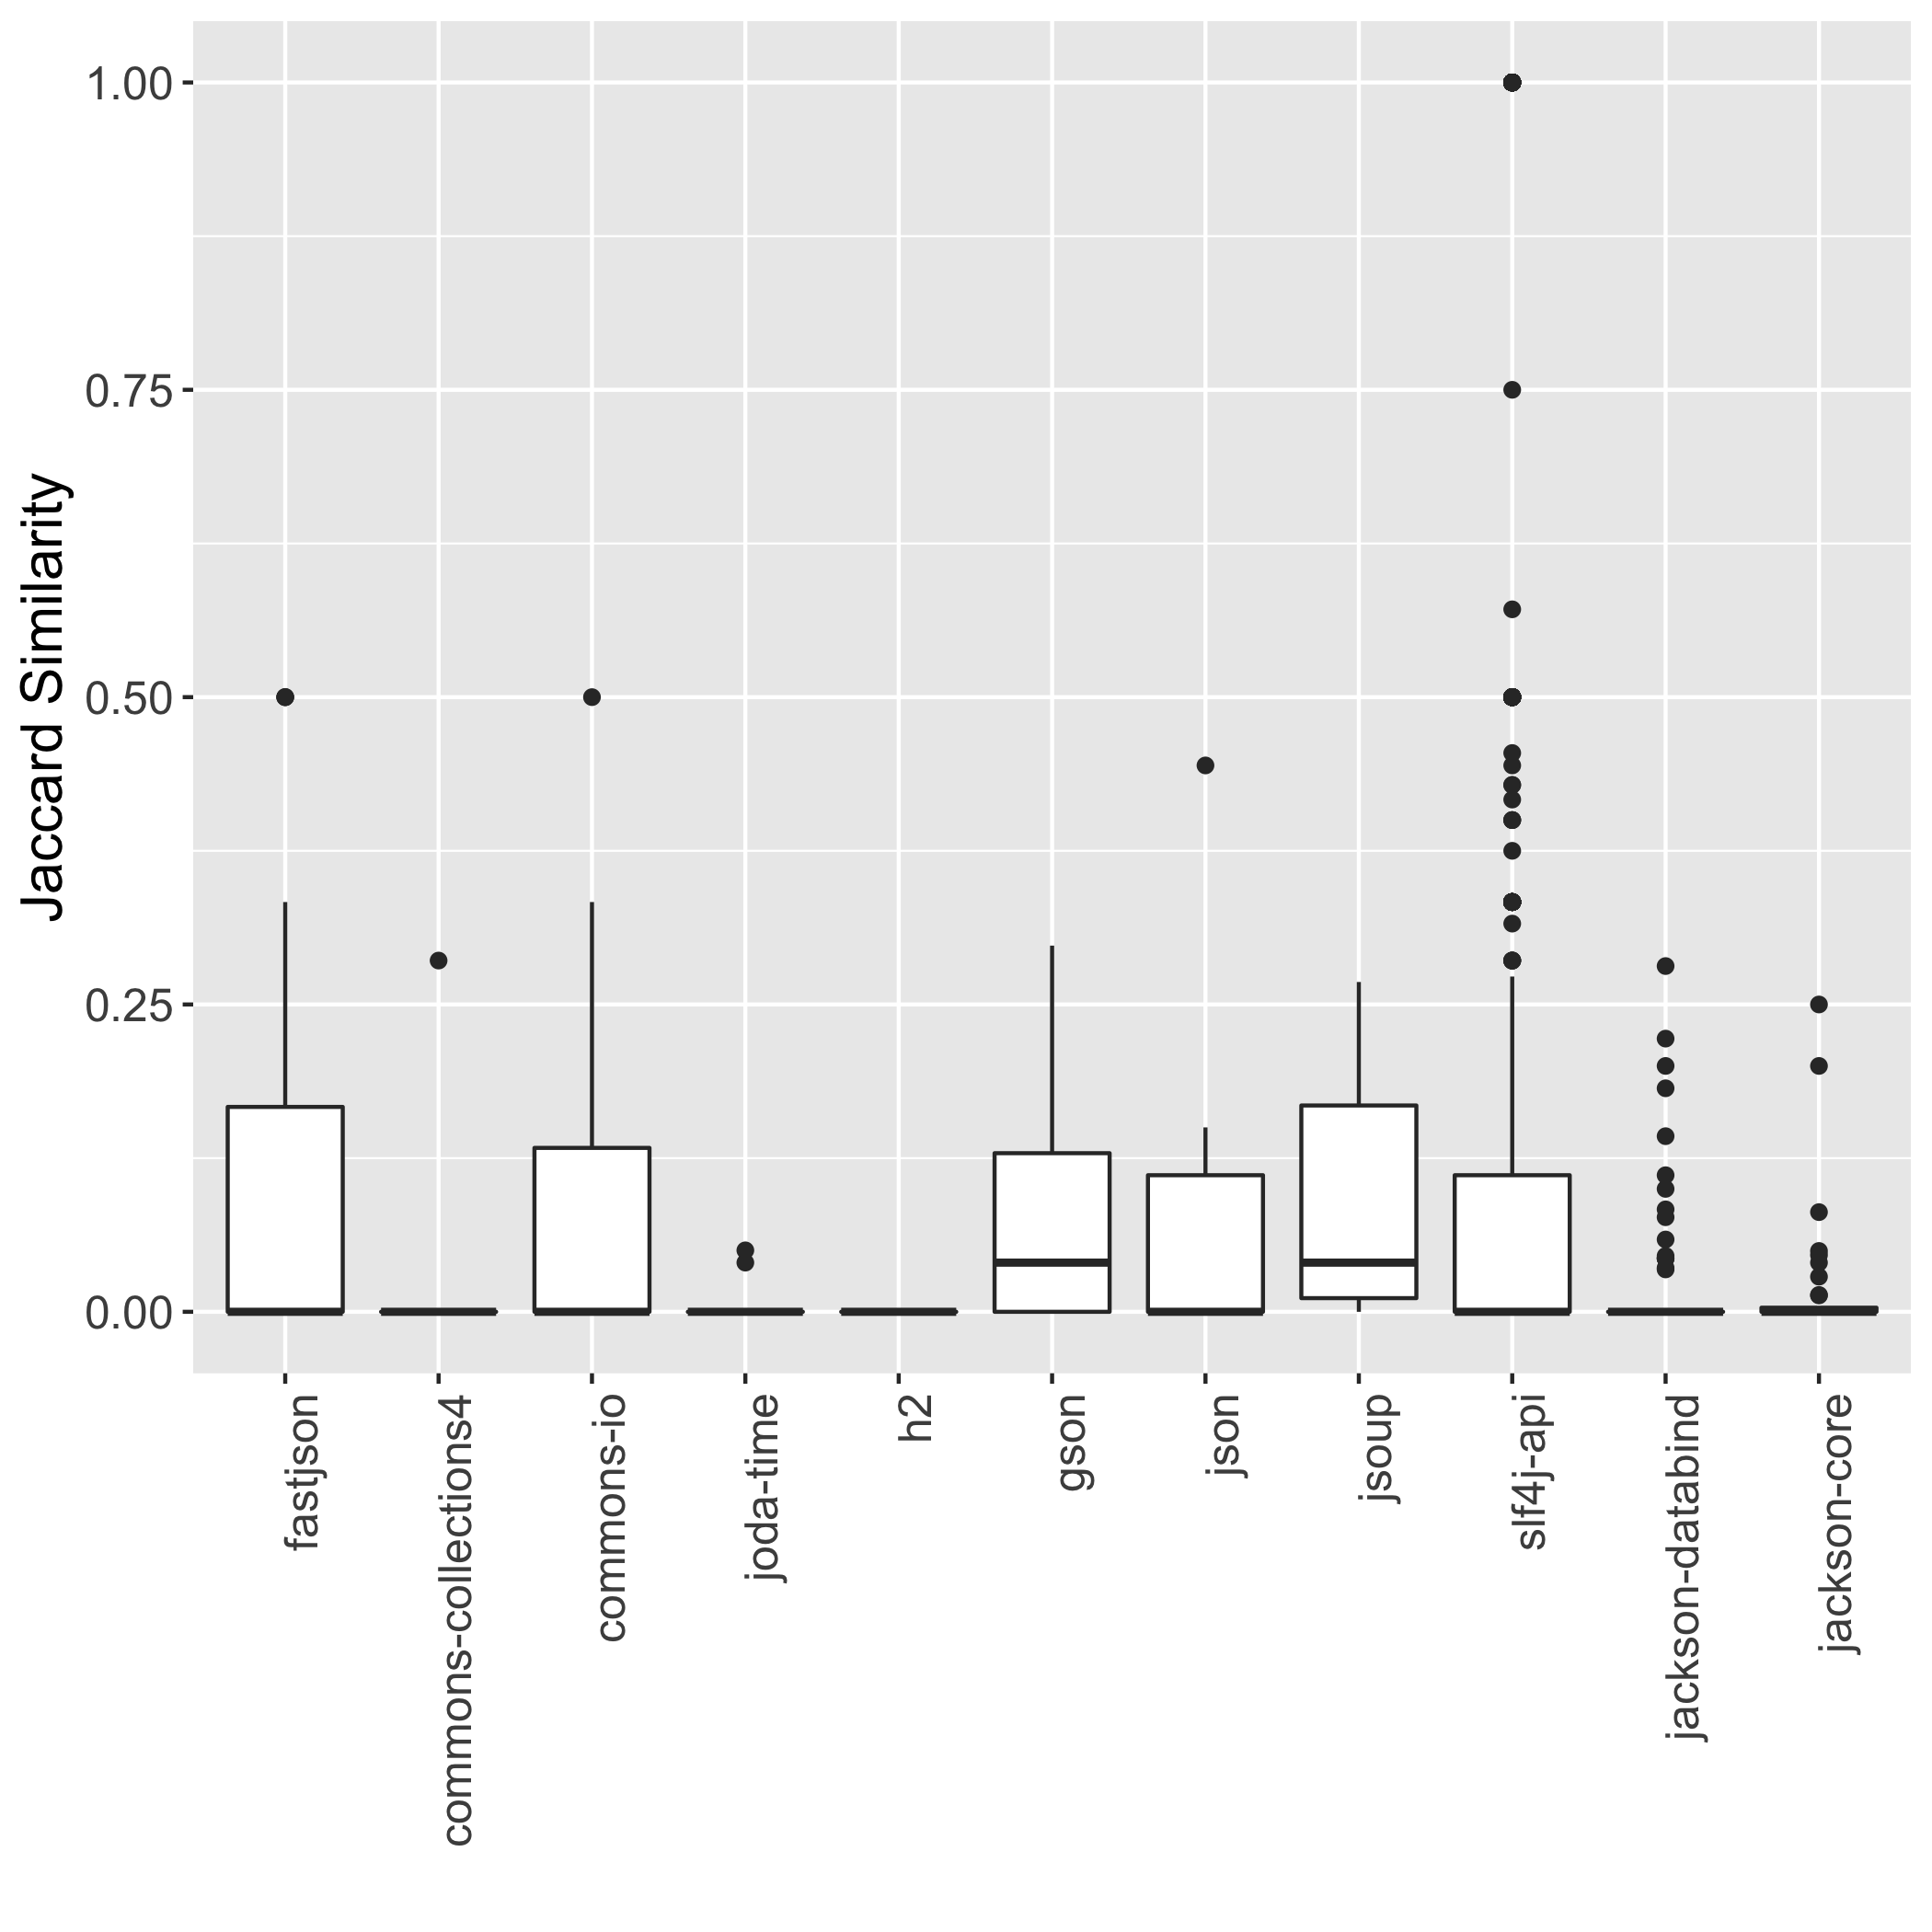
\includegraphics[width=8cm, height=7cm]{./images/jac-sim-box-plot-declared}
\caption{\label{fig:jaccard}Jaccard similarities between clients' API usages}
\end{figure}
\end{center}
%% Digging into \emph{fastjson}, we found that it is a ``mixed type'' library: some clients use APIs related
%% to \texttt{javax.ws.rs}, the JEE standard for restful services, while others use just a standalone parser API that does not implement an external specification. 

We were not surprised by the generally small amounts of overlap, because the libraries' exposed API surfaces tended
to have thousands of exposed elements and hundreds of used elements. This result makes a convincing argument for libraries being fissioned into modules, which we discuss further in Section~\ref{sec:fission}. 

Table~\ref{tab:same-method} presents another view of API overlap between clients. We constructed the largest set
of methods shared by more than 1 client of a library (``max-set'') and report the size of that set as well as the percentage
of clients which use all of that set of methods. So, for \emph{json}, we can see that there is one method called
by 3 out of 4 clients, and for \emph{jsoup}, ten methods are all called
by 3 out of 4 clients. We characterize the amount of overlap as generally low but not
nonexistent: a few methods are repeatedly used.

%\input{tables/results/perc-clients-same-methods}

%{\bf Research Question 2.} (a) Do clients often use only a subset of the published API? How big is this subset? (b) For each library, is that subset consistent across clients? (c) Do different libraries show different usage patterns by clients?

\begin{mdframed}[
  leftmargin=\parindent,
  rightmargin=\parindent,
  skipabove=\topsep,
  skipbelow=\topsep
  ]
{\bf Finding 2:} APIs are sparsely used by clients---mostly methods (9\% utilization), but a few fields (4\%) and supertypes (6\%). There is limited but nonzero overlap between the methods used by different clients.
\end{mdframed}

\section{Potential Applications}
\label{sec:potential-applications}
While the main contribution of this paper is to share our experiences
about writing program analysis and transformation tools, we also
briefly outline some potential applications of VizAPI itself.

In our original paper, we discussed how 1) library developers could
use VizAPI to guide their API maintenance decisions---based on actual
usage, which APIs were best prunable or modifiable, and where good
refactoring candidates might exist, thus helping library users'
experiences; and 2) client developers could use VizAPI to guide
decisions about when to upgrade their dependencies while avoiding
upgrade pains.

An extension of VizAPI could help with the problem of library selection. In
Section~\ref{sec:design-decisions} we discussed considerations for library
selection for VizAPI-like tools. An extension to VizAPI could also help
general developers pick which libraries would be helpful for their
needs---''projects like you used libraries X and Y''. In particular,
VizAPI can help surface the specific packages that similar projects used,
helping developers understand the functionalities of candidate libraries.

Our static and dynamic analyses record versions of different libraries used. 
Examining the data to observe how often clients upgrade library versions, 
whether clients use multiple versions of the same library is possibly interesting research for library developers.
\todo{library version usage: does this make sense?}

Another area of potential applications would be security; we already
identify {\texttt ServiceLoader} bypasses, and could also identify
other suspicious patterns. VizAPI would be particularly good for
identifying cases where vulnerabilities from dependencies do and do
not propagate; lack of an edge from a vulnerability-containing source
to a sink in a client would be a hint that the client would not be
vulnerable to the vulnerability. Unexpected edges could also indicate
abnormal behaviours that should be further investigated.
VizAPI could detect violations of
security policies, though it is admittedly not the best tool for that.

More fundamentally, we believe that the way VizAPI combines static and
dynamic information could be useful in understanding the limitations
of static and dynamic approaches in practice. In
Section~\ref{sec:design-decisions}, we talked about conceptual
limitations of both approaches. Sui et
al~\cite{sui20:_recal_static_call_graph_const_pract} have investigated
the recall of static call graph construction in practice, but further
work in this area would help in terms of having confidence in the
analysis results that we compute and rely on.

%% Potential Applications:
%% Security: 
%% Identify illegal accesses and abnormal usage
%% Identify propagated vulnerabilities from dependencies
%% Developer experience: analyze dataset for improving experience of library users
%% Help library developers identify which features to focus efforts on
%% Predict good choices of libraries based on client use case
%% Analyze library version usage: how often clients upgrade their library versions, do they use 
%% How does static and dynamic usage differ?
%% (other ML applications of the data??)

\section{Conclusion}
In this work, we have discussed the design and implementation of our
VizAPI artifact. VizAPI collects static and dynamic information
about interactions between components (clients, libraries, and dependencies) and makes
it visible to developers. We hope that our discussions will be of value
to future researchers who are looking to design static and dynamic
code analysis and visualization tools. 

\paragraph{Funding} This work was supported in part by Canada's Natural Science and Engineering Research Council.



%% The Appendices part is started with the command \appendix;
%% appendix sections are then done as normal sections
%% \appendix

%% \section{}
%% \label{}

%% References
%%
%% Following citation commands can be used in the body text:
%% Usage of \cite is as follows:
%%   \cite{key}         ==>>  [#]
%%   \cite[chap. 2]{key} ==>> [#, chap. 2]
%%

%% References with BibTeX database:

\bibliographystyle{elsarticle-num}
\bibliography{main}


\end{document}

%%
%% End of file `ecrc-template.tex'. 
